% Todas as linhas precedidas pelo simbolo '%' são comentários
% e não afetam em nada o seu texto final.

% IGNORE. Pacotes necessários e acessórios para o documento
\documentclass[12pt]{exam}
 \usepackage{graphicx}
\usepackage{amsthm}
\usepackage{libertine}
\usepackage[utf8]{inputenc}
\usepackage[margin=1in]{geometry}
\usepackage{amsmath,amssymb}
\usepackage{multicol}
\usepackage[brazil]{babel}
\usepackage[shortlabels]{enumitem}
% ---

% Informações que podem ser configuradas
% ---
\newcommand{\class}{Monitoria de cálculo L1A} % Nome da disciplina
\newcommand{\term}{2024}              % Perído Letivo
\newcommand{\examdate}{31/01/2024}        % insere a data no documento
\newcommand{\timelimit}{}               % IGNORE
\newcommand{\euler}{e}
% ---



\begin{document} % declaração de que o documento começa aqui.
\pagestyle{plain}
\thispagestyle{empty}
% ... formatação do cabeçalho
\noindent
\begin{tabular*}{\textwidth}{l @{\extracolsep{\fill}} r @{\extracolsep{6pt}} l}
 \textbf{\class} & \textbf{Monitor:} & \textit{Eduardo Guimarães}\\             % Insira o seu nome dentro dos {}'.
\textbf{\term} &&\\
\textbf{\examnum} &&\\
\textbf{\examdate} &&\\
\end{tabular*}\\
\rule[2ex]{\textwidth}{2pt}
% ---


\section{Máximos e Mínimos}


\begin{questions}
    \question Estude a função dada com relação a máximos e mínimos locais e globais.
    \begin{multicols}{1}
        \begin{enumerate}[(a)]
            \item
            $\displaystyle f(x) = e^x - e^{-3x} $
            \item 
            $\displaystyle g(x) = 2x^3 - 9x^2 + 12x + 3 $
            \item 
            $\displaystyle f(x) = x^2 + 3x + 2 $
            \item 
            $\displaystyle x(t) = t\cdot e^{-t}$
            \item 
            $\displaystyle y = e^{\displaystyle\frac{x-1}{x^2}}$
            \item 
            $\displaystyle g(x) = x^4 - 4x^3 + 4x^2 + 2 $
        \end{enumerate}
    \end{multicols}

    \question Determine as dimensões do retângulo de área máxima e cujo perímetro 2p é dado.

    \question Determine a altura do cone circular reto, de volume máximo, e com geratriz \textit{a} dada.

    
    \question Considere a curva $\displaystyle y = 1 - x^2 $,  para $x \in [0,1] $. Traçar uma tangente à
curva tal que a área do triângulo que ela forma com os eixos
coordenados seja mínima.

    
    \question Encontre o ponto da curva $\displaystyle y = \frac{2}{x} $ para x $>$ 0, que está mais próximo da origem.
    
    
    \question Do ponto A, situado numa das margens de um rio, de 100 m de largura, deve-se levar energia elétrica ao ponto C situado na outra margem do rio. O fio a ser utilizado na água custa R\$ 5 o metro, o que será utilizado fora, R\$ 3 o metro. Como deverá ser feita a ligação para que o gasto com os fios 
 seja o menor possível? (Suponha as margens retilíneas e paralelas.)

\begin{figure}[h]
    \centering
    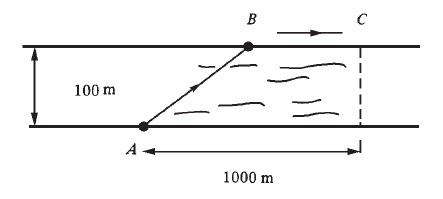
\includegraphics[width=10cm]{Screenshot 2024-01-30 162142.png}
    \caption{Figura questão 6}
    \label{fig:enter-label}
\end{figure}


\end{questions}

\end{document}
